\documentclass[12pt]{report}
\usepackage[a4paper, left=2cm, right=2cm]{geometry}
\usepackage{xcolor}
\definecolor{grey}{rgb}{0.9,0.9,0.9}
\usepackage[utf8]{inputenc}
\usepackage[T1]{fontenc}
%\usepackage[sfdefault]{ClearSans}
\usepackage[sfdefault,light]{FiraSans}
%\usepackage{XCharter} % Use the XCharter font (serif)
\usepackage{graphicx}
\usepackage{colortbl}
\usepackage{enumerate}

\renewcommand{\theenumii}{\theenumi.\arabic{enumii}}
\renewcommand{\labelenumi}{\theenumi.}
\renewcommand{\labelenumii}{\theenumii.}
\renewcommand{\contentsname}{Spis treści}
\usepackage{hyperref}
\hypersetup{
	colorlinks,
	citecolor=black,
	filecolor=black,
	linkcolor=black,
	urlcolor=black
}
\renewcommand{\chaptername}{}


\begin{document}
	\begin{titlepage} 
		\begin{center}
			
\includegraphics[scale=0.4]{agh.jpg}
		\end{center}

	\vfill
		\colorbox{grey}{
			\parbox[t]{0.93\textwidth}{
				\parbox[t]{0.91\textwidth}{
					\raggedleft
					\fontsize{50pt}{80pt}\selectfont
					\vspace{0.7cm}
					CoffeeLand\\
					\fontsize{20pt}{50pt}\selectfont
					Projekt sklepu internetowego\\
					\fontsize{15pt}{30pt}\selectfont
					Inżynieria Oprogramowania\\
					\vspace{0.7cm}
					
				}
			}
		}
	
		\vfill
		\parbox[t]{0.93\textwidth}{
			\raggedleft
			\large
			{\Large Aneta Pociecha}\\[4pt]
			{\Large Magdalena Tragarz}\\[4pt]
			{\Large Marek Ochocki}\\[4pt]
			{\Large Artur Bugaj}\\[4pt]
			\hfill\rule{0.2\linewidth}{1pt}\\[12pt]
			{Prowadzący zajęcia: dr inż. Marek Zachara}\\[4pt]
		}	
	\end{titlepage}
	
	%---------------------------------------------------------
	
	\newpage
	
	\tableofcontents

	\setcounter{chapter}{0}	
	\setcounter{section}{0}	
	

%---------------------------------------
%---------------------------------------
%---------------------------------------	
	\chapter{Streszczenie działania systemu}
	
	\section{Cel systemu}
	
		\paragraph{}
		
		Celem realizowanego systemu jest stworzenie prostego w użyciu sklepu internetowego z kawą. Zakupy wymagają założenia konta. Wybór produktów odbywa się poprzez katalog znajdujący się na stronie głównej. Klikając na produkt można przejść do osobnej strony ze szczegółowymi informacjami. Dodawanie produktów do koszyka odbywa się z poziomu podstrony produktu. W koszyku klient ma możliwość złożenia zamówienia. Płatność jest realizowana poprzez system PayPal. W sklepie Coffee Land został przewidziany system reklamacji.
	
	\section{Opis funkcjonalności z punktu widzenia klienta}
		
		\subsection{Wejścia systemu}
					\begin{itemize}
						\item formularz rejstracji 
						\item formularz logowania
						\item filtracja po typie kawy i cenie
						\item wprowadzenie danych adresowych
						\item formularz reklamacji
						\item edycja danych w profilu
						\item zapis do newslettera
					\end{itemize}

	
	\subsection{Lista możliwości}
		\begin{itemize}
			\item rejstracja użytkownika
			\item logowanie użytkownika
			\item zakup produktu
			\item reklamacja
			\item filtrowanie oferty ze względu na typ produktu i zakres ceny
			\item zapis do newslettera
			\item rezygnacja z newslettera
			\item dodanie adresu do listy adresów
			\item usunięcie adresu z listy adresów
			\item edycja danych użytkownika
		\end{itemize}


	\section{Opis funkcjonalności z punktu widzenia pracownika}

	\subsection{Wejścia systemu}
		\begin{itemize}
			\item 
			\item 
			\item
		\end{itemize}
	
	
	\subsection{Lista możliwości}
	\begin{itemize}
		\item 
		\item 
		\item
	\end{itemize}

%---------------------------------------
%---------------------------------------	
%---------------------------------------	
	\chapter{Diagram kontekstowy}

	\begin{center}
			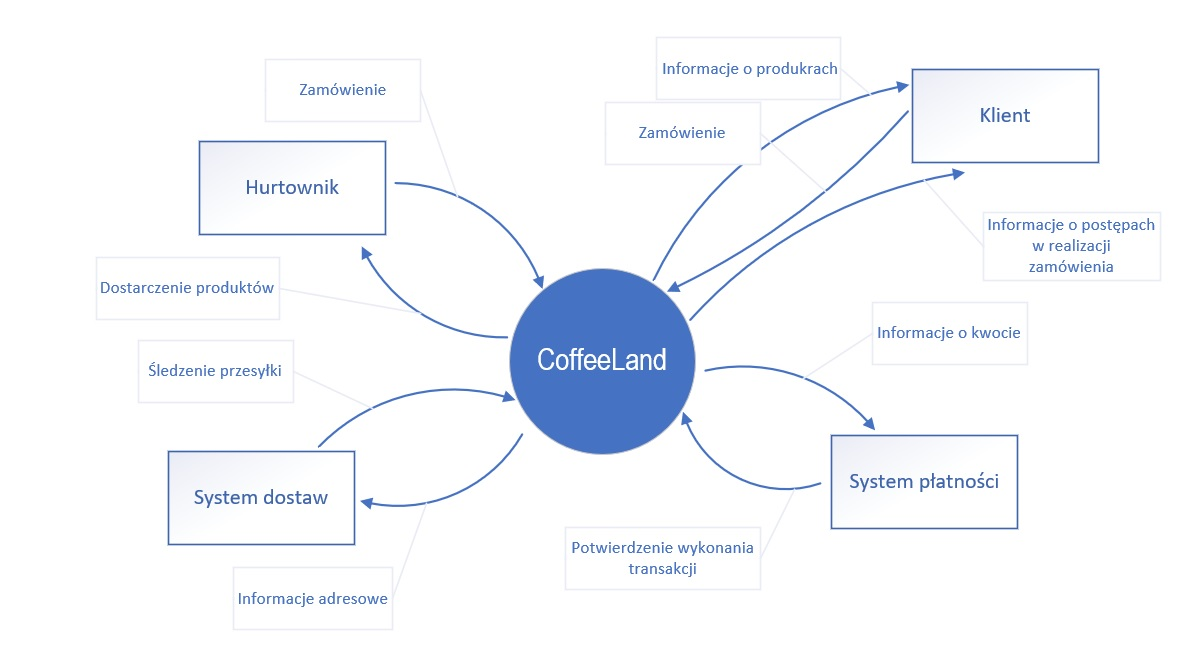
\includegraphics[scale=0.6]{kontekstowy.png}
	\end{center}

%---------------------------------------	
%---------------------------------------
%---------------------------------------
	
	\chapter{Funkcjonalności}
	\section{Rejstracja}
	
%---------------------------------------
	\begin{table}[h]
		\def\arraystretch{1.3}
		\begin{tabular}{|>{\columncolor[gray]{0.97}}p{4cm}| p{12cm} |}
			\hline
			\textbf{Aktorzy}		
					& Użytkownik 			\\ \hline
			\textbf{Zakres}    		
					& Sklep internetowy     \\ \hline
			\textbf{Poziom}     	
					& Sytemowowy            \\ \hline
			\textbf{Udziałowcy i cele}	
					& Użytkownik chce stworzyć konto. Sklep chce zebrać dane spełniające zadane warunki.           					\\ \hline
			\textbf{\begin{tabular}[l]{@{}l@{}}Zdarzenie \\ wyzwalające\end{tabular}} 	
					& Użytkownik przechodzi na podstronę ‘Sign in/Register’ 														\\ \hline
			\textbf{Warunki wstępne}	
					& brak 																											\\ \hline
			\textbf{\begin{tabular}[l]{@{}l@{}}Warunki końcowe \\ dla sukcesu\end{tabular}}     
					& Konto użytkownika zostaje utworzone i zapisane w bazie danych. Użytkownik zostaje powiadomiony o sukcesie.  	\\ \hline
			\textbf{\begin{tabular}[l]{@{}l@{}}Warunki końcowe \\ dla niepowodzenia\end{tabular}}   
					& Konto nie zostaje stworzone. Użytkownik zostaje powiadomiony o niepowodzeniu i przyczynach niepowodzenia. 	\\ \hline
		\end{tabular}
	\end{table}
%---------------------------------------
	\colorbox{grey}{Scenariusz główny:}
		\begin{enumerate}
			\item System wyświetla formularz wprowadzania danych rejestracji
			\item Użytkownik wprowadza dane (zdefiniowane w słowniku): imię, nazwisko, email, hasło
			\item System weryfikuje dane
			\item System wyświetla powiadomienie o udanej rejestracji
		\end{enumerate}
%---------------------------------------	
	
	\colorbox{grey}{Scenariusz alternatywny:}
		\begin{enumerate}\addtocounter{enumi}{2}
			\item[]
			\begin{enumerate}
				\item Nie wprowadzono wymaganych danych
				\begin{enumerate}
					\item System wyświetla ponownie formularz zaznaczając, które dane powinny zostać poprawione i jakie warunki powinny spełniać zaznaczone dane
					\item Następuje powrót do punktu 2 scenariusza głównego
				\end{enumerate}
			\end{enumerate}
		\end{enumerate}
%---------------------------------------

	\colorbox{grey}{Scenariusz alternatywny:}
	\begin{enumerate}\addtocounter{enumi}{2}
		\item[]
		\begin{enumerate}
			\item W bazie danych znajduję się konto dla podanego email’a
			\begin{enumerate}
				\item System wyświetla ponownie formularz zaznaczając email i wyświetla informację o istnieniu konta dla podanego email’a
				\item Następuje powrót do punktu 2 scenariusza głównego
			\end{enumerate}
		\end{enumerate}
	\end{enumerate}

%---------------------------------------
%---------------------------------------
%---------------------------------------

	\section{Logowanie}
	\begin{table}[h]
		\def\arraystretch{1.3}
		\begin{tabular}{|>{\columncolor[gray]{0.97}}p{4cm}| p{12cm} |}
			\hline
			\textbf{Aktorzy}		
			& Użytkownik 			\\ \hline
			\textbf{Zakres}    		
			& Sklep internetowy     \\ \hline
			\textbf{Poziom}     	
			& Sytemowowy            \\ \hline
			\textbf{Udziałowcy i cele}	
			& Użytkownik chce się zalogować. Sklep chce zebrać dane spełniające zadane warunki.           					\\ \hline
			\textbf{\begin{tabular}[l]{@{}l@{}}Zdarzenie \\ wyzwalające\end{tabular}} 	
			& Użytkownik przechodzi na podstronę ‘Sign in/Register’ 														\\ \hline
			\textbf{Warunki wstępne}	
			& brak 																											\\ \hline
			\textbf{\begin{tabular}[l]{@{}l@{}}Warunki końcowe \\ dla sukcesu\end{tabular}}     
			& Użytkownik zastaje zalogowany. Następuje przekierowanie na podstronę 'Shop'. 	\\ \hline
			\textbf{\begin{tabular}[l]{@{}l@{}}Warunki końcowe \\ dla niepowodzenia\end{tabular}}   
			& Użytkownik nie zostaje zalogowany. Użytkownik zostaje powiadomiony o niepowodzeniu. 	\\ \hline
		\end{tabular}
	\end{table}

	%---------------------------------------
	\colorbox{grey}{Scenariusz główny:}
	\begin{enumerate}
		\item System wyświetla formularz wprowadzania danych logowania
		\item Użytkownik wprowadza dane: email, hasło
		\item System weryfikuje czy w bazie danych istnieje konto, które odpowiada wprowadzonym danym
		\item System przekierowuje na podstronę ‘Shop’.
		\item System wyświetla ‘My account’ na pasku nawigacji
		\item System zamienia opcję przekierowania na postronę ‘Sign in/Register’ na opcję wylogowania użytkownika ‘Sign out’
		\item Użytkownik przechodzi na podstronę ‘My account’
		\item Użytkownik wybiera opcję ‘Sign out’
		\item System przekierowuje na podstonę ‘Shop’
		\item System usuwa ‘My account’ z paska nawigacji
	\end{enumerate}
	%---------------------------------------	
	
	\colorbox{grey}{Scenariusz alternatywny:}
	\begin{enumerate}\addtocounter{enumi}{3}
		\item[]
		\begin{enumerate}
			\item Nie istnieje konto dla wprowadzonych danych
			\begin{enumerate}
				\item System wyświetla informację o niepowodzeniu
				\item Następuje powrót do punktu 2 scenariusza głównego
			\end{enumerate}
		\end{enumerate}
	\end{enumerate}
	%---------------------------------------
	
	\colorbox{grey}{Scenariusz alternatywny:}
	\begin{enumerate}\addtocounter{enumi}{6}
		\item[]
		\begin{enumerate}
			\item Następuje przejście do punktu 9 scenariusza głównego
		\end{enumerate}
	\end{enumerate}

	%---------------------------------------	
	\colorbox{grey}{Scenariusz alternatywny:}
	\begin{enumerate}\addtocounter{enumi}{8}
		\item[]
		\begin{enumerate}
			\item Następuje przejście do punktu 10 scenariusza głównego
		\end{enumerate}
	\end{enumerate}
	
%---------------------------------------		
	\section{Wylogowanie}
%---------------------------------------
\newpage
		
	\section{Zmiana zawartości koszyka}
		\subsection{Dodawanie produktów do koszyka z poziomu podstrony produktu}
		
		\begin{table}[h]
			\def\arraystretch{1.3}
			\begin{tabular}{|>{\columncolor[gray]{0.97}}p{4cm}| p{12cm} |}
				\hline
				\textbf{Aktorzy}		
				& Użytkownik 			\\ \hline
				\textbf{Zakres}    		
				& Sklep internetowy     \\ \hline
				\textbf{Poziom}     	
				& Sytemowowy            \\ \hline
				\textbf{Udziałowcy i cele}	
				& Użytkownik chce dodać produkty do koszyka. Sklep chce zebrać i zapisać informacje o zawartości koszyka.           					\\ \hline
				\textbf{\begin{tabular}[l]{@{}l@{}}Zdarzenie \\ wyzwalające\end{tabular}} 	
				& Użytkownik przechodzi na podstronę produktu. 														\\ \hline
				\textbf{Warunki wstępne}	
				& brak 																											\\ \hline
				\textbf{\begin{tabular}[l]{@{}l@{}}Warunki końcowe \\ dla sukcesu\end{tabular}}     
				& Dodanie produktu do koszyka.	\\ \hline
				\textbf{\begin{tabular}[l]{@{}l@{}}Warunki końcowe \\ dla niepowodzenia\end{tabular}}   
				& Stan koszyka nie zostaje zmieniony. Użytkownik zostaje powiadomiony o niepowodzeniu. 	\\ \hline
			\end{tabular}
		\end{table}
		
		%---------------------------------------
		\colorbox{grey}{Scenariusz główny:}
		\begin{enumerate}
			\item System wyświetla podstronę produktu
			\item Użytkownik wprowadza ilość produktów
			\item System weryfikuje dane 
			\item Użytkownik wybiera opcję 'Add to Cart'
			\item System zmienia stan koszyka
		\end{enumerate}
		%---------------------------------------	
		
		\colorbox{grey}{Scenariusz alternatywny:}
		\begin{enumerate}\addtocounter{enumi}{3}
			\item[]
			\begin{enumerate}
				\item Ilość nie jest liczbą naturalną
				\begin{enumerate}
					\item System wyświetla ponownie formularz zaznaczając które dane powinny zostać poprawione
					\item Następuje powrót do punktu 2 scenariusza głównego
				\end{enumerate}
			\end{enumerate}
		\end{enumerate}
		%---------------------------------------
		
	\subsection{Zmiana zawartości koszyka z poziomu podstrony koszyka}
	
	\begin{table}[h]
		\def\arraystretch{1.3}
		\begin{tabular}{|>{\columncolor[gray]{0.97}}p{4cm}| p{12cm} |}
			\hline
			\textbf{Aktorzy}		
			& Użytkownik 			\\ \hline
			\textbf{Zakres}    		
			& Sklep internetowy     \\ \hline
			\textbf{Poziom}     	
			& Sytemowowy            \\ \hline
			\textbf{Udziałowcy i cele}	
			& Użytkownik chce zmienić zawartość koszyka. Sklep chce zaktualizować informacje o zawartości koszyka.           					\\ \hline
			\textbf{\begin{tabular}[l]{@{}l@{}}Zdarzenie \\ wyzwalające\end{tabular}} 	
			& Użytkownik przechodzi na podstronę koszyka. 														\\ \hline
			\textbf{Warunki wstępne}	
			& brak 																											\\ \hline
			\textbf{\begin{tabular}[l]{@{}l@{}}Warunki końcowe \\ dla sukcesu\end{tabular}}     
			& Aktualizacja stanu koszyka.	\\ \hline
			\textbf{\begin{tabular}[l]{@{}l@{}}Warunki końcowe \\ dla niepowodzenia\end{tabular}}   
			& Stan koszyka nie zostaje zmieniony. Użytkownik zostaje powiadomiony o niepowodzeniu. 	\\ \hline
		\end{tabular}
	\end{table}
	
	%---------------------------------------
	\colorbox{grey}{Scenariusz główny:}
	\begin{enumerate}
		\item System wyświetla podstronę produktu
		\item Użytkownik zmienia ilość produktów
		\item System weryfikuje dane 
		\item Użytkownik wybiera opcję 'Update Cart'
		\item System aktualizuje stan koszyka
	\end{enumerate}
	%---------------------------------------	
	
	\colorbox{grey}{Scenariusz alternatywny:}
	\begin{enumerate}\addtocounter{enumi}{3}
		\item[]
		\begin{enumerate}
			\item Ilość nie jest liczbą naturalną
			\begin{enumerate}
				\item System wyświetla ponownie formularz zaznaczając które dane powinny zostać poprawione
				\item Następuje powrót do punktu 2 scenariusza głównego
			\end{enumerate}
		\end{enumerate}
	\end{enumerate}
	%---------------------------------------
	
%---------------------------------------			
	\section{Zakup produktu}
	\section{Reklamacja}	
	\section{Filtrowanie produktów}
	\section{Zapis do newslettera}
	\section{Rezygnacja z newslettera}
	\section{Dodanie adresu do listy adresów}
	\section{Usunięcie adresu z listy adresów}
	\section{Edycja danych użytkownika}
		
	
	
%---------------------------------------	

	\renewcommand{\thesection}{\thechapter.\arabic{section}}		
	
	\chapter{Model danych - diagramy ERD}

	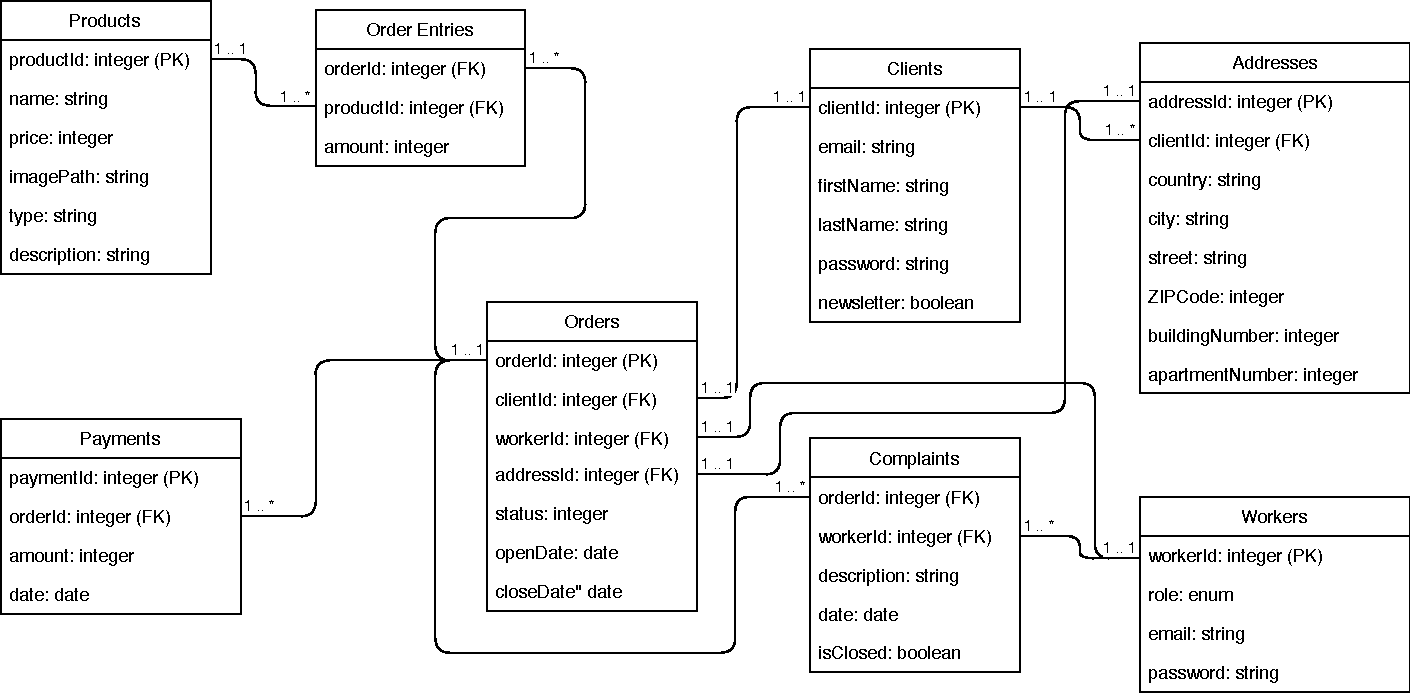
\includegraphics[width=500pt]{database.jpg}
	
	
%---------------------------------------	
	\chapter{Model dynamiki - diagramy STD}
	
%---------------------------------------	
	\chapter{Specyfikacja procesów PSPEC}
	
	
%---------------------------------------	
	\chapter{Słownik danych}
	
%---------------------------------------	
	\chapter{Technologie i narzędzia}	
		\section{Technologie}
		\begin{itemize}
			\item JavaScript
			\item SignalR
			\item React
			\item nUnit
			\item .NET
			\item JestTest
			\item CircleCI
		\end{itemize}
		
		\section{Narzędzia}
		\begin{itemize}
			\item Visual Studio Code
			\item Visual Studio Community
			\item Selenium
			\item Chromium
		\end{itemize}
	
\end{document}